Reinforcement learning (RL) algorithms provide for an automated framework for decision making and control: by specifying a high-level objective function, an RL algorithm can, in principle, automatically learn a control policy that satisfies this objective. 
This has the potential to automate a range of applications, such as autonomous vehicles and interactive conversational agents. 
However, current model-free reinforcement learning  algorithms are quite expensive to train, which often limits their application to simulated domains~\citep{Mnih2015,Lillicrap2016,schulman2017proximal}, with a few exceptions~\citep{Kober2009,Levine2016}. 
A promising direction for reducing sample complexity is to explore model-based reinforcement learning~(MBRL) methods, which proceed by first acquiring a predictive model of the world, and then using that model to make decisions~\citep{Atkeson1997,Kocijan2004,Deisenroth2014}. 
MBRL is appealing because the dynamics model is reward-independent and therefore can generalize to new tasks in the same environment, and it can easily benefit from all of the advances in deep supervised learning to utilize high-capacity models. 
However, the asymptotic performance of MBRL methods on common benchmark tasks generally lags behind model-free methods. That is, although MBRL methods tend to learn more quickly, they also tend to converge to less optimal solutions.

In this paper, we take a step toward narrowing the gap between model-based and model-free RL methods. 
Our approach is based on several observations that, though relatively simple, are critical for good performance. 
We first observe that model capacity is a critical ingredient in the success of MBRL methods: while efficient models such as Gaussian processes can learn extremely quickly, they struggle to represent very complex and discontinuous dynamical systems~\citep{Calandra2016a}. 
By contrast, neural network (NN) models can scale to large datasets with high-dimensional inputs, and can represent such systems more effectively. 
However, NNs struggle with the opposite problem: to learn fast means to learn with few data and NNs tend to overfit on small datasets, making poor predictions far into the future. 
For this reason, MBRL with NNs has proven exceptionally challenging.

Our second observation is that this issue can, to a large extent, be mitigated by properly incorporating uncertainty into the dynamics model. 
While a number of prior works have explored uncertainty-aware deep neural network models~\citep{neal1995bayesian,Lakshminarayanan2017}, including in the context of RL~\citep{Gal2016,Depeweg2016}, our work is, to our knowledge, the first to bring these components together in a deep MBRL framework that reaches the asymptotic performance of state-of-the-art model-free RL methods on benchmark control tasks. 

\begin{figure}[t]
	\centering
	
	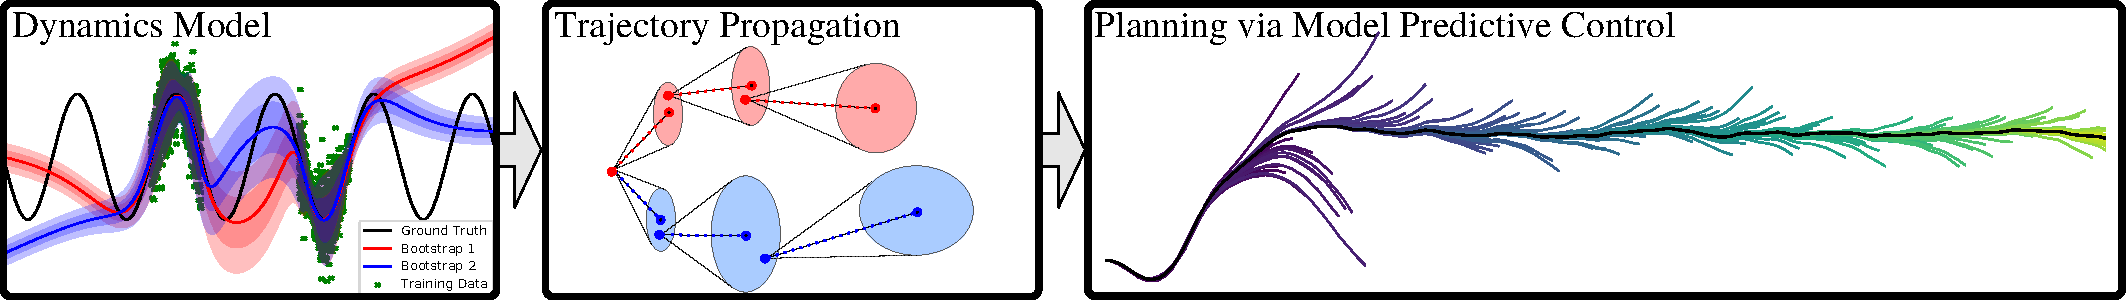
\includegraphics[width=\linewidth]{fig/diagram.pdf}
	\caption{Our method (PE-TS):
	\textbf{Model}: Our probabilistic ensemble (PE) dynamics model is shown as an ensemble of two bootstraps (bootstrap disagreement far from data captures epistemic uncertainty: our subjective uncertainty due to a lack of data), each a probabilistic neural network that captures aleatoric uncertainty (inherent variance of the observed data).
	\textbf{Propagation}: Our trajectory sampling (TS) propagation technique uses our dynamics model to re-sample each particle (with associated bootstrap) according to its probabilistic prediction at each point in time, up until horizon~$\horizon$.
	\textbf{Planning}: At each time step, our MPC algorithm computes an optimal action sequence, applies the first action in the sequence, and repeats until the task-horizon.
	}
	\label{fig:diagram}
\end{figure}

Our main contribution is an MBRL algorithm called probabilistic ensembles with trajectory sampling (PETS)\footnote{Code available \url{https://github.com/kchua/handful-of-trials}} summarized in \fig{fig:diagram} with high-capacity NN models that incorporate uncertainty via an ensemble of bootstrapped models, where each model encodes \textit{distributions} (as opposed to point predictions), rivaling the performance of model-free methods on standard benchmark control tasks at a fraction of the sample complexity.
An advantage of PETS over prior probabilistic MBRL algorithms is an ability to isolate two distinct classes of uncertainty: aleatoric (inherent system stochasticity) and epistemic (subjective uncertainty, due to limited data). Isolating epistemic uncertainty is especially useful for directing exploration~\citep{thrun1992efficient}, although we leave this for future work.
Finally, we present a systematic analysis of how incorporating uncertainty into MBRL with NNs affects performance, during both model training and planning.
We show, that PETS' particular treatment of uncertainty significantly reduces the amount of data required to learn a task, e.g., eight times fewer data on half-cheetah compared to the model-free Soft Actor Critic algorithm~\citep{Haarnoja2018softUpdated}.

